% !TEX encoding = UTF-8
% 第六章（解读）：X-SAM 消融——逃逸属于全局分量
% 对应论文 §5.3（Only SAM escapes; the X-SAM ablation）与图 28。

\section{X-SAM 消融：逃逸属于全局分量}
\label{sec:ch06}

\begin{keybox}{本章速览}
\begin{itemize}
  \item 问题：X-SAM（Duan 等，2026）在 SAM 上叠加秩-1 顶部特征向量修正，
        声称``显式约束 $\lmax$''；论文检验该修正是否有可检测的贡献。
  \item 四臂对比：CIFAR-10/ResNet-18、确定性 CUDA、$n{=}10$——
        SGD / SAM($\rho{=}0.05$) / faithful X-SAM（Duan Eq.~11：
        固定 $\alpha{=}0.2$、无钳位、符号门控、每步触发）/ clamped 变体
        （$d=\max(\hat\lambda/(2/\eta),1)$）。
  \item 晚期（步 $\geq3000$）真 $\lmax$：SGD $31.1\pm2.3$、SAM
        $23.3\pm1.6$、faithful $23.9\pm1.6$、clamped $23.4\pm1.6$
        ——三个 SAM 族 CI 重叠。
  \item 配对差（paired difference，同种子配对相减再统计：两臂共享同一
        种子的难度与数据噪声，相减后这些共同波动被约掉、只剩优化器本身
        的差异——同样的种子数能分辨更小的效应）$\Delta\lmax(\text{faithful}-\text{SAM})=+0.62\pm1.23$
        （晚期）、$+0.59\pm2.55$（中期），CI 均跨零；晚期效应量上界
        $+1.85$（效应量 = 真实差异的大小；上界即其 CI 上端——真实差异
        再大也大不过它），小于 SAM 晚期绝对 $\lmax$ 的 $\sim8\%$。
  \item 测量纪律：ARPACK 真 $\lmax$（确定性 512 样本批、$k{=}3$、
        $\mathrm{tol}{=}10^{-6}$）；小批幂迭代在该交叉熵海森上伪收敛
        （平均低估 $+45\%$，实测）。
\end{itemize}
\end{keybox}

\paragraph{本章在论文中的位置。}
本章对应论文 §5.3。第 \ref{sec:ch05} 章建立的机制排序——proxy 帽与单方向
plant 都不下逃逸、只有 SAM 全局动作下行——在这里变成对第三方方法的
\emph{可证伪检验}：如果排序正确，那么任何``SAM $+$ 单方向修正''的组合，其
逃逸都应来自 SAM 分量，修正本身不应有可检测的贡献。X-SAM（Duan 等，2026）
正是这样一个组合，且作者声称其修正``显式约束 $\lmax$''——这是一个直接
冲突，必须实测。本章的副产品——钳位门控可以制造休眠——直接催生第
\ref{sec:ch07} 章的 clamp-free 桥；本章确立的确定性噪声地板标准，后来也用来
重验规模实验的三向排序（解读第八章）。

\subsection{问题设定：把机制排序变成可证伪检验}
\label{sec:ch06-question}

X-SAM $=$ SAM 的全局扰动
（$\varepsilon=\rho\,\mathbf{g}/\|\mathbf{g}\|$，Foret 等 2021）
$+$ 沿 top 特征向量的秩-1 梯度修正——结构上正是``全局动作 $+$ 第
\ref{sec:ch05} 章的秩-1 plant''。Duan 等 (2026) 的框架是``显式约束
$\lmax$''。论文的机制猜想（第 \ref{sec:ch05} 章 C3 的两体制结论）预言：
骑在 SAM 上的秩-1 修正不应有超越 SAM 的可检测贡献；孤立的秩-1 修正（无
SAM 底座）在 MLP 测试床上不仅起不到约束作用，反而会按体制 (ii) 上逃逸。如果
faithful X-SAM 显著低于 SAM，机制排序就要修正——所以这是一个真正可证伪
的检验，而不是走过场的消融。

\subsection{四臂设计与测量纪律}
\label{sec:ch06-design}

\paragraph{四臂。}CIFAR-10/ResNet-18，\emph{确定性} CUDA 模式，$n{=}10$
种子：
\begin{itemize}
  \item \textbf{SGD}：基线；
  \item \textbf{SAM}（$\rho{=}0.05$）：全局扰动底座；
  \item \textbf{faithful X-SAM}：忠实实现 Duan 等 Eq.~11——固定
        $\alpha{=}0.2$（此 $\alpha$ 为 Duan 算法的固定修正幅度超参，
        与第五章的梯度分量 $\alpha=\langle\mathbf{g},\hat v\rangle$
        无关）、无钳位、符号门控（sign-gated，只取内积
        $\langle g,v\rangle$ 的正负号、不管其大小，来决定修正的方向）、无条件每步触发；
  \item \textbf{clamped 变体}：$d=\max(\hat\lambda/(2/\eta),1)$——即论文
        自家 C3 门控的保守消融臂。
\end{itemize}

\paragraph{测量纪律一：CUDA 非确定性。}
默认的 conv 反向传播是非确定的：两个完全相同的 SAM run 会发散到
$\sim10^{-1}$ 的终态参数差，产生 $\sim6$ 单位的伪 $\lmax$ 差距——若不
加控制，跨优化器的单种子 $\lmax$ 比较会被 CUDA 噪声主导。确定性模式消除
之。这是本章的第一条方法论教训：\emph{在比较 $\lmax$ 之前先证明两个相同
 run 逐位重合}。

\paragraph{测量纪律二：估计器伪收敛。}
小批幂迭代估计在该交叉熵海森上\emph{伪收敛}（false convergence）——平均
低估 $+45\%$（直接实测的数字）。因此论文报告 ARPACK 真 $\lmax$：确定性
512 样本批、$k{=}3$、$\mathrm{tol}{=}10^{-6}$。这与论文预测端的主题呼应：
便宜的锐度估计器有明确的失效区，用它测量之前必须先诊断——同一教训在规模
实验（解读第八章）里还会以更大的代价重演一次。

\subsection{结果：null——三个 SAM 族臂不可区分}
\label{sec:ch06-result}

\paragraph{真 $\lmax$。}
晚期（步 $\geq3000$）、$n{=}10$、mean$\pm95\%$ CI：
\begin{center}
\begin{tabular}{lc}
\toprule
优化器 & 晚期真 $\lmax$ \\
\midrule
SGD & $31.1\pm2.3$ \\
SAM & $23.3\pm1.6$ \\
faithful X-SAM & $23.9\pm1.6$ \\
clamped X-SAM & $23.4\pm1.6$ \\
\bottomrule
\end{tabular}
\end{center}
三个 SAM 族臂的 CI 重叠。配对差
$\Delta\lmax(\text{faithful}-\text{SAM})$ 为 $+0.62\pm1.23$（晚期）、
$+0.59\pm2.55$（中期）——两个 CI 都跨零。晚期效应量上界 $+1.85$（CI
上界）：\emph{在该功效（statistical power，检出给定大小效应的能力：
种子越少、噪声越大，功效越低、只能检出大效应——故``检测不到''不等于``效应为零''；本设计 $n{=}10$、配对差半宽 $\pm1.23$，等价于把大于
$+1.85$ 的效应排除在 95\% 置信之外——这就是``该功效''的定量内容）下，任何低于 SAM 的秩-1 降压都小于 SAM 晚期绝对
$\lmax$ 的 $\sim8\%$（$1.85/23.3\approx7.9\%$；区间 $[-0.61,+1.85]$
同时界住了\emph{有利}方向：任何降压效应至多 $0.61\approx$ SAM 水平
的 $2.6\%$）。}

\paragraph{精度。}
$n{=}10$ 终精度：SGD $0.802$、SAM $0.817$、faithful $0.814$、clamped
$0.815$（都在 $\pm0.02$ CI 内）。faithful X-SAM 不在 SAM 之上——反而低
$0.3$ 点。锐度上检测不到的贡献，也没有带来任何精度增益。

\paragraph{两个补充事实钉死``逃逸属于全局分量''。}
其一，SAM 在该 CIFAR-10 设置下比 SGD 低 $\sim8$ 单位（CIFAR-100 三向差
$\sim7$，见解读第八章），无论秩-1 修正是否骑在上面。其二，孤立的 rank-1
（无 SAM 底座）在第 \ref{sec:ch05} 章的 MLP 测试床上不是约束器而是帽移除
器——上逃逸到 $261.8\pm5.4$（体制 (ii)）。合起来：单独使用时它把帽向上
移除；骑在 SAM 上时贡献低于确定性噪声地板（论文用语，未单独给出数值
——定性指确定性协议下剩余的种子噪声尺度；与之相对，第~\ref{sec:ch03-determinism}~节的
非确定性 CUDA 伪差距约 $6$ 单位，配对差半宽为 $\pm1.23$）。逃逸\emph{压倒性地}是全局 SAM
分量。

\begin{figure}[!ht]
\centering
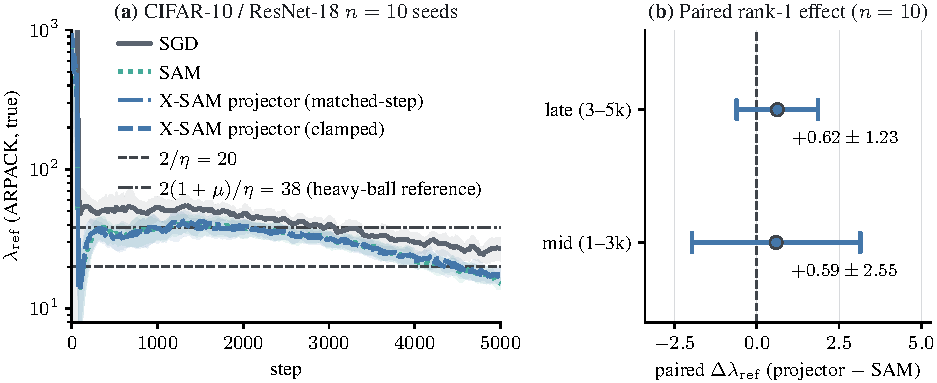
\includegraphics[width=0.95\linewidth]{28_xsam_ablation.pdf}
\caption{X-SAM 消融（论文图 28）：CIFAR-10/ResNet-18，$n{=}10$ 确定性种子，
ARPACK 真 $\lmax$。(a) $\lmax$ 轨迹（粗线为种子均值、阴影为 $95\%$ CI）：
SAM、faithful X-SAM、clamped X-SAM 都降到 SGD 之下，且
faithful$\approx$clamped$\approx$SAM。(b) 配对差
$\Delta\lmax(\text{faithful}-\text{SAM})$（中期与晚期）：CI 均跨零
（晚期 $+0.62\pm1.23$、上界 $+1.85$）——该功效下检测不到秩-1 修正对
$\lmax$ 的效应。孤立 rank-1 消融（无 SAM 底座；MLP 测试床）上逃逸到
$\lmax=261.8\pm5.4$（正文）。}
\label{fig:ch06-xsam}
\end{figure}

\subsection{对 Duan 协议的三点偏离（忠实性声明）}
\label{sec:ch06-fidelity}

论文明确：这是受控的 $\lmax$-\emph{动力学}比较，不是对方精度基准的复现。
Duan 等 (2026) 的设置：CIFAR-10/ResNet-18、SGD 底座、cosine lr $0.1$、
weight decay $5{\times}10^{-5}$、批 $256$、$200$ epochs、flip/pad/crop
增强、$\rho{=}0.05$、$\alpha{=}0.2$、$3$ runs；他们在该设置下报告 X-SAM
$94.71\pm0.20$ vs SAM $93.64\pm0.30$，以及跨 CIFAR-10 骨干 $+1.21\%$
平均 / $+2.08\%$ 最大。三点偏离：

\begin{enumerate}
  \item \textbf{梯度归一化}：他们的 Alg.~2 沿\emph{单位化的}修正梯度更新
        ——步长与损失尺度解耦，修正效应与每步学习率的变化混淆。本文的
        faithful 臂把符号门控投影
        $P_t=I-\alpha\,\mathrm{sign}(\langle g,v\rangle)\,vv^{\top}$
        （即其 Eq.~11 修正）施加于\emph{原始}对抗梯度，使有效步长 $\eta$
        在 SGD/SAM/X-SAM 之间匹配——否则比较的不是修正本身，而是一次隐蔽
        的调 lr。
  \item \textbf{日程}：$5000$ 步（$\approx13$ epochs）、恒定 lr $0.1$、
        批 $128$、weight decay $5{\times}10^{-4}$、无增强、确定性 CUDA
        ——为 $n{=}10$ 的种子级可复现而选，而非峰值精度；对方的精度数字
        出自 200 epoch 增强食谱，与本设置不可直接对比。
  \item \textbf{特征向量刷新}：热启动幂迭代、每步 5 次 HVP、HVP 期间冻结
        BN 统计——比对方的间歇估计更新鲜；若修正有效应，这里的版本只会
        \emph{更强}。
\end{enumerate}

\subsection{null 结果的含义与边界}
\label{sec:ch06-interpretation}

\paragraph{含义。}
在 matched-$\eta$ 动力学（matched-$\eta$ dynamics，各臂有效步长被对齐后的公平动力学比较）下，秩-1 修正对 $\lmax$ 与精度的贡献都检测不到
（晚期上界 $+1.85$，$<8\%$）；``显式约束 $\lmax$''的表述不被支持。第
\ref{sec:ch05} 章的机制排序由此从猜想升级为实测：逃逸属于全局分量。

\paragraph{边界（诚实清单）。}
其一，这个界只覆盖 matched-$\eta$ 动力学——对方 Alg.~2 的归一化更新未测
；其二，全协议复现（cosine 日程、增强、归一化更新、200 epochs）仍是
gap；其三，null 是``在此功效下检测不到''，不是``效应为零''——效应量上界
$+1.85$ 就是这句话的定量形式。

\paragraph{副产品 $\to$ 第 \ref{sec:ch07} 章。}
消融暴露了一个尴尬的自家问题：clamped 臂的秩-1 修正 $0\%$ 步触发，而
faithful $100\%$——$\max(\cdot,1)$ 钳位可以\emph{制造休眠}（dormant）。
而论文的 at-scale 秩-1 plant 用的是同一个钳位，其``惰性''判定——触发比例（fired fraction，执行器实际发挥作用的步数占比）
$\le4\%$、$\approx$SGD——部分是基于这个观察作出的——它也因此沾上了同样
的嫌疑：也许真正中和它的是钳位、不是景观。这个怀疑必须正面处理，就是第
\ref{sec:ch07} 章的
clamp-free 桥。

\subsection*{本章要点}
\begin{itemize}
  \item \textbf{null 结果}（null result，在给定统计功效下检测不到差异的阴性结果）：晚期真 $\lmax$ 三个 SAM 族臂 CI 重叠
        （$23.3\pm1.6$ / $23.9\pm1.6$ / $23.4\pm1.6$）；配对差
        $+0.62\pm1.23$（晚期）、$+0.59\pm2.55$（中期）均跨零；效应量上界
        $+1.85<\text{SAM 晚期绝对 }\lmax$ 的 $8\%$。
  \item \textbf{精度同样不分}：$0.802$/$0.817$/$0.814$/$0.815$
        （$\pm0.02$ CI 内），faithful 比 SAM 低 $0.3$ 点。
  \item \textbf{逃逸属于全局分量}：SAM 比 SGD 低 $\sim8$ 单位与秩-1
        修正无关；孤立 rank-1 在 MLP 上反而上逃逸到 $261.8\pm5.4$。
  \item \textbf{测量纪律}：CUDA 非确定性可制造 $\sim6$ 单位伪差距（须确定性
        模式）；小批幂迭代在该海森上伪收敛、平均低估 $+45\%$（须 ARPACK）。
  \item \textbf{边界}：界只覆盖 matched-$\eta$ 动力学；全协议复现仍是
        gap；副产品——钳位可制造休眠——催生第 \ref{sec:ch07} 章的
        clamp-free 桥。
\end{itemize}
